% ----------------------------------------------------------
% Introdução (exemplo de capítulo sem numeração, mas presente no Sumário)
% ----------------------------------------------------------
\chapter{Introdução}
% ----------------------------------------------------------

A inteligência artificial (IA) vem ganhando manchetes no mundo todo,sendo anunciada tanto como uma salvação econômica quanto como precursora de desintegração social. Quando computadores programáveis foram concebidos pela primeira vez, as pessoas se perguntavam se essas máquinas poderiam se tornar inteligentes, mais de cem anos antes de uma ser construída.
% \cite{menabrea1843sketch}.
 Hoje, a inteligência artificial é um campo com inúmeras aplicações práticas e tópicos de pesquisa ativos. Buscamos softwares inteligentes para automatizar o trabalho de rotina, entender a fala ou as imagens, fazer diagnósticos em medicina e apoiar a pesquisa científica \cite{Goodfellow-et-al-2016}.


A IA adiciona inteligência a produtos existentes. Na maioria dos casos, a inteligência artificial não é vendida como uma aplicação individual. Pelo contrário, produtos já existentes são aprimorados com funcionalidades de IA, de maneira parecida como a Siri foi adicionada aos produtos da \textit{Apple}. Automação, plataformas de conversa, robôs e aparelhos inteligentes podem ser combinados com grandes quantidades de dados para aprimorar diversas tecnologias para casa e escritório, de inteligência em segurança à análise de investimentos.

A maioria dos exemplos de IA sobre os quais se ouve falar hoje – de computadores mestres em xadrez a carros autônomos – dependem de \textit{deep learning} e processamento de linguagem natural (PNL) \cite{pln-o-que-e}. Treinar um agente para superar os jogadores humanos e otimizar sua performance pode nos ensinar como otimizar diferentes processos em uma grande variedade de situações. Foi o que o \textit{DeepMind} do Google fez com seu popular \textit{AlphaGo} e seu sucessor \textit{AlphaZero}, vencendo os campeões mundiais em Go, xadrez e shogi, e obtendo resultados de performance nunca antes vistos.

\section{Motivação}

Técnicas de aprendizado de máquina e algoritmos de \textit{deep learning} têm consistentemente melhorado a capacidade de um computador de fornecer reconhecimento de padrões e previsões cada vez mais precisas. Além disso, sistemas de DL são consistentemente aplicados com sucesso a conjuntos de aplicações cada vez mais amplos.

Ao mesmo tempo em que a escala e a precisão das redes profundas aumentaram, a complexidade das tarefas que podem ser resolvidas também cresceu significativamente. 
Uma conquista importante de sistemas de DL é a sua extensão ao domínio da aprendizagem por reforço (\textit{reinforcement learning}) \cite{reinforcement-learning-intro-2018}. No contexto do aprendizado por reforço, um agente autônomo deve aprender a executar uma tarefa por tentativa e erro, sem nenhuma orientação do operador humano. 

Além do valor para pesquisa em múltiplas áreas da ciência, muitas dessas aplicações de aprendizado de máquina e \textit{deep learning} são altamente lucrativas. O aprendizado de máquina hoje é usado por muitas empresas de tecnologia, incluindo \textit{Google, Microsoft, Facebook}, IBM, \textit{Baidu, Apple, Adobe, Netflix}.

Diante à crescente presença de sistemas que utilizam técnicas de \textit{deep learning} no dia-a-dia, nota-se o grande potencial do investimento em pesquisa, modelagem de novos problemas e estudo de técnicas de aprendizado de máquina. 
%
Uma interessante aplicação desses sistemas está na área de jogos digitais. A indústria de videogames tem testemunhado um enorme crescimento, graças, em boa parte, ao incrível aumento no poder da computação em termos de representações visuais. 
%
%
Seja no controle de personagens não-jogadores (NPC), ou para a geração de conteúdo processual (PCG), são inúmeras as potenciais aplicações dessas técnicas em jogos digitais.
%
O potencial dessas ferramentas de obter uma vantagem competitiva no mercado, ou simplesmente fornecer uma melhor experiência para o usuário é, no mínimo, instigante.
%
Nesse contexto, a modelagem de novos problemas, implementação de soluções utilizando técnicas de \textit{deep learning} e investimento na área, torna-se uma relevante contribuição para o estado da arte.


\section{Objetivos}
 O presente trabalho tem como objetivo geral propor o desenvolvimento de uma IA capaz de aprender a jogar diferentes jogos, desde que se tenha acesso ao código fonte e feito em Allegro. Para isso, será implementado um algoritmo utilizando \textit{Deep Reinforcement Learning}, abordagem que consiste em fornecer ao sistema parâmetros relacionados ao seu estado e uma recompensa positiva ou negativa com base em suas ações. 
 % Nenhuma regra sobre o jogo é dada e, inicialmente, a IA não tem informações sobre o que precisa fazer. A única informação passada para a IA são os comandos básicos do jogo. 
 O objetivo do sistema é descobrir e elaborar uma estratégia para maximizar a pontuação - ou a recompensa.
 % Diferente de muitas IAs que focam na solução de um único problema, a proposta deste projeto é elaborar uma IA que seja genérica e capaz solucionar e elaborar estratégias para uma variedade de situações diferentes.

 Os objetivos mais específicos deste trabalho são:
 \begin{enumerate}
 	\item Revisão da literatura do problema;
 	\item Descrição e modelagem do problema;
 	\item Proposta de critérios adicionais que possibilitem estimar outras características das possíveis soluções do projeto, tais como performance, confiabilidade, entre outras;
 	\item Proposta de um algoritmo de \textit{deep learning} para a solução do problema;
 	\item Análise dos resultados obtidos em comparação com diferentes soluções implementadas por outras entidades e utilizadas na prática por empresas atuando no mercado.
 \end{enumerate}

 Perante o exposto, a implementação de algoritmos que utilizam o aprendizado de máquina de forma a serem aplicados em diferentes cenários,
 apresenta um potencial de propor novas estratégias e otimizar sistemas já existentes, melhorar a qualidade do produto final e a experiência do usuário, além de proporcionar uma vantagem competitiva no mercado.

\section{Descrição do problema}
O campo da inteligência artificial é capaz de solucionar, com certa facilidade, problemas que são intelectualmente muito difíceis para os serem humanos, mas relativamente diretos para os computadores - problemas que podem ser descritos por uma lista de regras formais e matemáticas. Tarefas abstratas e formais que estão entre os empreendimentos mentais mais difíceis para um ser humano estão entre os mais fáceis para um computador.

Ironicamente, o grande desafio à inteligência artificial provou estar em resolver tarefas fáceis de executar para um ser humano. Problemas  que parecem automáticos, que resolvemos intuitivamente, como reconhecer palavras faladas ou rostos em imagens. Os computadores há muito conseguem derrotar até o melhor jogador de xadrez humano \cite{Hsu:2002:BDB:601291}, mas apenas recentemente começaram a alcançar algumas das habilidades dos seres humanos comuns, como reconhecer objetos ou fala. 

A vida cotidiana de uma pessoa requer uma imensa quantidade de conhecimento sobre o mundo. A grande quantidade de informação desses cenários torna inviável a codificação de todas as regras do sistema e, por isso, o computador tem uma grande dificuldade para solucionar esses problemas. Além disso, grande parte desse conhecimento é subjetivo e intuitivo e, portanto, difícil de articular de maneira formal. Os computadores precisam capturar esse mesmo conhecimento para se comportarem de maneira inteligente. Um dos principais desafios da inteligência artificial é como obter esse conhecimento informal em um computador.

As dificuldades enfrentadas por sistemas que dependem de conhecimento codificado sugerem que os sistemas de IA necessitam da capacidade de adquirir seu próprio conhecimento, extraindo padrões de dados brutos. Esse recurso é conhecido como aprendizado de máquina ou \textit{machine learning} (ML). A introdução do aprendizado de máquina permitiu que os computadores resolvessem problemas que envolvem o conhecimento sobre o mundo real e tomassem decisões mais subjetivas.

 No contexto de jogos digitais, treinar um agente para superar os jogadores humanos e otimizar sua pontuação pode nos ensinar como otimizar processos diferentes em uma variedade de subcampos diferentes e intrigantes \cite{comi:teach:AI:DRL:2018}. Uma abordagem proposta na literatura, obtendo ótimos resultados, e que tem como objetivo treinar um computador pra aprender e desenvolver estratégias para jogar diferentes jogos, é o \textit{deep reinforcement learning}.

 O problema proposto nesse trabalho é o de implementar uma IA que, utilizando algoritmos de \textit{deep reinforcement learning}, seja capaz de aprender e desenvolver estratégias para jogar diferentes jogos digitais. Os requisitos do sistema podem ser resumidos pelos seguintes critérios:
\begin{enumerate}
	\item O sistema receberá, inicialmente, somente os comandos básicos do jogo. Nenhuma regra sobre o jogo é dada e, inicialmente, o agente não tem nenhuma informação sobre o que precisa fazer;
	\item O agente deve ser capaz de elaborar uma estratégia para maximizar sua pontuação e que alcance resultados consideravelmente superiores aos de uma abordagem aleatória e próximos aos de um agente humano;
	\item O sistema deverá ser capaz de lidar com cenários aleatórios, onde os obstáculos mudam a cada partida, e não aleatórios, onde os obstáculos são ``fixos'' e a dificuldade varia de acordo com o progresso no jogo;
	\item O sistema deve ser generalizado para que possa ser aplicado à diferentes cenários e treinado para jogar diferentes jogos digitais.
\end{enumerate}

De modo a garantir a factibilidade da implementação do sistema, algumas restrições devem ser acatadas. Por exemplo, além de haver a necessidade de se conhecer os comandos básicos do jogo, o sistema precisa ser capaz de obter informações atualizadas sobre o estado do jogo em que se encontra. No caso deste trabalho, foram definidas as seguintes restrições:

\begin{enumerate}
	\item O sistema deve ter acesso ao código fonte do jogo no qual será aplicado;
	\item O jogo deverá ter sido implementado em \textit{Allegro}\footnote{O acesso ao código fonte nos permite ter conhecimento dos comandos básicos do jogo, enquanto a biblioteca \textit{Allegro} permite a manipulação de algumas variáveis como a velocidade com que os estados do jogo são atualizados.};
	\item O jogo deve ser 2D;
\end{enumerate}



\subsection{\textit{Deep Learning}}


 O \textit{deep learning} (DL) é uma área do aprendizado de máquina que propõe que os computadores aprendam com a experiência, se ajustem à novas entradas de dados e compreendam o mundo em termos de hierarquia de conceitos, sendo cada conceito definido por sua relação com conceitos mais simples. 
 Ao reunir conhecimento a partir da experiência, essa abordagem evita a necessidade dos operadores humanos de especificar formalmente todo o conhecimento que o computador precisa. Além disso, a hierarquia de conceitos permite que o computador aprenda conceitos complexos, construindo-os a partir de conceitos mais simples. Isso nos permite treinar os computadores para cumprir tarefas específicas ao processar grandes quantidades de dados e reconhecer padrões nesses dados.

 A \textbf{Figura \ref{hierarquia-conceitos-dl}} mostra como um sitema de \textit{deep learning} representa o conceito de imagem de uma pessoa combinando conceitos mais simples, como cantos e contornos, que por sua vez são definidos em termos de arestas. 
 O mapeamento de funções de um conjunto de pixels para uma identidade de objeto é muito complicado. O algoritmo de \textit{deep learning} resolve essa dificuldade dividindo o mapeamento complicado desejado em séries de mapeamentos simples aninhados, cada um deles descrito por uma camada diferente do modelo. A entrada é apresentada na camada visível, assim denominada porque contém as variáveis que podemos observar.
 Em seguida, uma série de camadas ocultas extrai recursos cada vez mais abstratos da imagem. Essas camadas são chamadas de "ocultas" porque seus valores não são fornecidos nos dados; em vez disso, o algoritmo deve determinar quais conceitos são úteis para explicar os relacionamentos nos dados observados. A camada de saída obtém a identidade de objeto abstrata a partir dos conceitos obtidos pelas camadas ocultas.


 \begin{figure}[h]
 \centering
 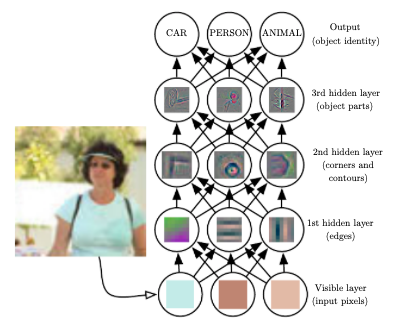
\includegraphics[width=.6 \textwidth]{conteudo/imgs/hierarquia-conceitos-dl.png}
 \caption[Ilustração de um modelo de aprendizado profundo]{Ilustração de um modelo de aprendizado profundo. Dados os pixels, a primeira camada pode identificar facilmente as bordas, comparando o brilho dos pixels vizinhos. Dada a descrição das arestas pela primeira camada oculta, a segunda camada oculta pode procurar facilmente cantos e contornos estendidos, reconhecíveis como coleções de arestas. Dada a descrição da segunda camada oculta da imagem em termos de cantos e contornos, o terceiro setor oculto pode detectar partes inteiras de objetos específicos, encontrando coleções específicas de contornos e cantos. Finalmente, esta descrição da imagem em termos das partes do objeto que ela contém pode ser usada para reconhecer os objetos presentes na imagem. Imagem retirada de \cite{Goodfellow-et-al-2016}}
 \label{hierarquia-conceitos-dl}
\end{figure}

\subsection{\textit{Reinforcement Learning}} % (fold)
\label{sub:reinforcement_learning}

O aprendizado por reforço ou \textit{reinforcement learning} (RL) é uma abordagem computacional para entender e automatizar o aprendizado direcionado a objetivos e a tomada de decisões. O aprendizado por reforço distingue-se de outras abordagens computacionais por sua ênfase na aprendizagem de um agente apartir da interação direta com seu ambiente, sem exigir supervisão exemplar ou modelos completos do ambiente \cite{reinforcement-learning-intro-2018}.

Em algoritmos de \textit{reinforcement learning}, o agente não é informado sobre quais ações executar, mas, em vez disso, deve descobrir quais ações geram mais recompensa, através de tentativa e erro. Em alguns casos mais interessantes, as ações podem afetar não apenas a recompensa imediata, mas também a próxima situação e, com isso, todas as recompensas subsequentes. Essas duas características - pesquisa por tentativa e erro e recompensa atrasada - são as duas características distintivas mais importantes do aprendizado por reforço.

% O aprendizado por reforço é diferente do aprendizado supervisionado, o tipo de aprendizado estudado na maioria das pesquisas atuais no campo do aprendizado de máquina. Aprendizado supervisionado é aprender com um conjunto de treinamento de exemplos rotulados fornecidos por um supervisor externo qualificado. O objetivo desse tipo de aprendizado é o sistema extrapolar ou generalizar suas respostas para que ele atue corretamente em situações não presentes no conjunto de treinamento.
%  % Este é um tipo importante de aprendizado, mas por si só não é adequado para aprender com a interação. Em problemas interativos, muitas vezes é impraticável obter exemplos do comportamento desejado que sejam corretos e representativos de todas as situações nas quais o agente precisa agir. Em um território desconhecido - onde se espera que a aprendizagem seja mais benéfica - um agente deve ser capaz de aprender com sua própria experiência.

%  O aprendizado por reforço também é diferente do que os pesquisadores de aprendizado de máquina chamam de aprendizado não supervisionado, que geralmente consiste em encontrar estruturas ocultas em coleções de dados não rotulados. Os termos aprendizado supervisionado e aprendizado não supervisionado parecem classificar exaustivamente os paradigmas de aprendizado de máquina, mas não o fazem. Embora se possa ficar tentado a pensar no aprendizado por reforço como um tipo de aprendizado não supervisionado, porque não se baseia em exemplos de comportamento correto, o aprendizado por reforço está tentando maximizar um sinal de recompensa em vez de tentar encontrar uma estrutura oculta. Descobrir a estrutura na experiência de um agente certamente pode ser útil no aprendizado por reforço, mas por si só não aborda o problema do aprendizado por reforço de maximizar um sinal de recompensa. Portanto, o aprendizado por reforço é considerado como um terceiro paradigma de aprendizado de máquina, ao lado de aprendizado supervisionado, aprendizado não supervisionado e talvez outros paradigmas  \cite{reinforcement-learning-intro-2018}.

Além do agente e do ambiente, é interessante ressaltar alguns elementos importantes de um sistema de aprendizado por reforço: a \textbf{política}, o \textbf{sinal de recompensa} e a \textbf{função de valor}.

A \textbf{política} define a maneira que o agente deve se comportar em um determinado momento. 
Uma política é basicamente um mapeamento dos estados do ambiente para as ações a serem tomadas quando nesses estados. 
A política em casos mais simples ter a forma de uma função simples ou uma tabela de pesquisa, enquanto em casos mais complexos pode envolver cálculos mais extensivos. 
Em geral, as políticas podem ser estocásticas, especificando probabilidades para cada ação.

Um \textbf{sinal de recompensa} define o objetivo de um problema de aprendizado por reforço. 
Em cada etapa, o ambiente envia ao agente de aprendizado por reforço um único número que funciona como uma recompensa para o agente. 
O único objetivo do agente é maximizar a recompensa total que recebe a longo prazo.
O sinal de recompensa define, portanto, quais são os eventos bons e ruins para o agente. 
O sinal de recompensa é a base principal para alterar a política - se uma ação selecionada pela política for seguida por uma baixa recompensa, a política poderá ser alterada para selecionar outra ação nessa situação no futuro. 
Em geral, os sinais de recompensa podem ser funções estocásticas do estado do ambiente e das ações tomadas.

Enquanto o sinal de recompensa indica o que é bom em um sentido imediato, uma \textbf{função de valor} especifica o que é bom a longo prazo. 
O valor de um estado representa a quantidade total de recompensa que um agente pode esperar acumular no futuro, a partir desse estado. 
Enquanto as recompensas determinam a conveniência imediata e intrínseca dos estados ambientais, os valores indicam a conveniência a longo prazo dos estados após levar em conta os estados que provavelmente seguirão e as recompensas disponíveis nesses estados. 
Por exemplo, um estado sempre pode gerar uma recompensa imediata baixa, mas ainda tem um valor alto porque é seguido regularmente por outros estados que produzem recompensas altas. Ou o contrário poderia ser verdade. 

A \textbf{Figura \ref{rl-diagram}} mostra um diagrama de aprendizagem por reforço relacionando o agente de aprendizado com o ambiente no qual ele é inserido.
O ambiente representa o mundo pelo qual o agente se move. O ambiente nada mais é do que um sistema que toma o estado atual e a ação do agente como entrada e retorna como saída a recompensa do agente e seu próximo estado. 

Ambientes podem ser modelados como funções que transformam uma ação executada no estado atual, no próximo estado e uma recompensa. Já os agentes podem ser modelados como funções que transformam o novo estado e recompensam na próxima ação. 
Podemos conhecer a função do agente, mas não podemos conhecer a função do ambiente. É uma caixa preta onde só vemos as entradas e saídas. 
% É como o relacionamento da maioria das pessoas com a tecnologia: sabemos o que faz, mas não sabemos como funciona. 
O aprendizado por reforço representa a tentativa de um agente de aproximar a função do ambiente, para que possamos enviar ações para o ambiente de caixa preta que maximize as recompensas que ele distribui \cite{beg-guide-rl}.

\begin{figure}[h]
 \centering
 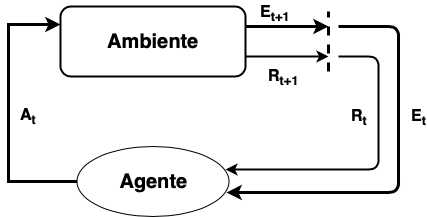
\includegraphics[width=.6 \textwidth]{conteudo/imgs/rl-diagram.png}
 \caption[Diagrama de aprendizagem por reforço]{Diagrama de aprendizagem por reforço. No \textit{loop} de \textit{feedback} acima, os subscritos indicam as etapas de tempo $t$ e $t + 1$, cada uma das quais se refere a estados diferentes: o estado no momento $t$ e o estado no momento $t + 1$. 
 % Diferente de outras formas de aprendizado de máquina - como aprendizado supervisionado e não supervisionado - o aprendizado por reforço só pode ser pensado sequencialmente em termos de pares de ação de estado que ocorrem um após o outro.
 A ação $A_t$ de um agente é determinada por sua \textbf{política}, que por sua vez é uma função que depende do estado atual do sistema $E_t$. A política de um agente tem como objetivo maximizar a \textbf{função de valor} que é calculada utilizando o \textbf{sinal de recompensa} $R_t$. O ambiente se comporta como um sistema caixa preta que transforma uma ação executada no estado atual $A_t$, no próximo estado $E_{t+1}$ e uma recompensa $R_{t+1}$
 }
 \label{rl-diagram}
\end{figure}

As escolhas de ação são feitas com base em julgamentos de valor.
Buscamos ações que gerem estados de maior valor, e não de maior recompensa, porque essas ações obtêm a maior quantidade de recompensa para nós a longo prazo. 
Infelizmente, é muito mais difícil determinar valores do que determinar recompensas. As recompensas são basicamente dadas diretamente pelo ambiente, mas os valores devem ser estimados e re-estimados a partir das sequências de observações que um agente faz ao longo de toda a sua vida útil.

% subsection reinforcement_learning (end)

\subsection{Aplicação de DRL no treinamento de uma IA para aprender a jogar jogos em \textit{Allegro}} % (fold)
\label{sub:aplicação_de_drl_no_treinamento_de_uma_ia_para_aprender_a_jogar_jogos_em_allegro}

% No contexto de jogos digitais, treinar um agente para superar os jogadores humanos e otimizar sua pontuação pode nos ensinar como otimizar processos diferentes em uma variedade de subcampos diferentes e intrigantes \cite{comi:teach:AI:DRL:2018}. Uma abordagem proposta na literatura, obtendo ótimos resultados, e que tem como objetivo treinar um computador pra aprender e desenvolver estratégias para jogar diferentes jogos, é o \textit{deep reinforcement learning}.

O \textit{deep reinforcement learning} (DRL) é uma abordagem do \textit{deep learning} que, em contraste a abordagens mais tradicionais como o aprendizado supervisionado e não supervisionado, utiliza as técnicas de aprendizagem por reforço para treinar o agente. Essa abordagem consiste em fornecer ao sistema parâmetros relacionados ao seu estado e uma recompensa positiva ou negativa com base em suas ações. Nenhuma regra sobre o jogo é dada e, inicialmente, o agente não tem nenhuma informação sobre o que precisa fazer. O objetivo do sistema é descobrir e elaborar uma estratégia para maximizar sua pontuação - ou recompensa.





% subsection aplicação_de_drl_no_treinamento_de_uma_ia_para_aprender_a_jogar_jogos_em_allegro (end)

\section{Revisão da literatura }

No contexto de \textit{reinforcement learning}, o \textit{DeepMind} demonstrou que um aprendizado por reforço, baseado no aprendizado profundo, é capaz de aprender a jogar videogames Atari, atingindo desempenho em nível humano em diversas tarefas \cite{mnih-human-control-drl}.

O \textit{deep learning} também contribuiu para outras ciências. As redes convolucionais modernas para reconhecimento de objetos fornecem um modelo de processamento visual que os neurocientistas podem estudar \cite{dicarlo-afrax-yamins:2014}. O \textit{deep learning} também fornece ferramentas úteis para processar grandes quantidades de dados e fazer previsões úteis em campos científicos. Ele tem sido usado com sucesso para prever como as moléculas irão interagir, a fim de ajudar as empresas farmacêuticas a projetar novos medicamentos \cite{dahl2014multitask}, a procurar partículas subatômicas \cite{baldi:s:w:2015}. Espera-se que o DL apareça em cada vez mais campos científicos no futuro.







